% ----
% COMP1204 CW2 Report Document
% ----

\documentclass[12pt,oneside,a4paper,english]{article}
\usepackage{listings}
\usepackage{xcolor}
\usepackage{sectsty}
\usepackage[margin=0.5in]{geometry}
\usepackage[font=small,labelfont=bf]{caption}

\usepackage{titlesec}
\titlespacing*{\subsection}
{0cm}{0.5cm}{0.3cm}

\usepackage{longtable}
\usepackage{booktabs}

\usepackage{graphicx}

%Change paragraphs font
\paragraphfont{\Large}

%Colors defined below
\definecolor{codegreen}{rgb}{0,0.6,0}
\definecolor{codegray}{rgb}{0.5,0.5,0.5}
\definecolor{codepurple}{rgb}{0.58,0,0.82}
\definecolor{backcolour}{rgb}{0.95,0.95,0.92}

%Code listing style
\lstdefinestyle{codestyle}{
  backgroundcolor=\color{backcolour}, commentstyle=\color{codegreen},
  keywordstyle=\color{magenta},
  numberstyle=\small\color{codegray},
  stringstyle=\color{codepurple},
  basicstyle=\ttfamily\normalsize,
  breakatwhitespace=false,
  breaklines=true,
  captionpos=b,
  keepspaces=true,
  numbers=left,
  numbersep=5pt,
  showspaces=false,
  showstringspaces=false,
  showtabs=false,
  tabsize=2
}

\lstset{style=codestyle}

\begin{document}
\title{COMP1204: Data Management \\ Coursework Two: COVID Cases Database }
\author{Daniel Braghis \\ 32161204}
\maketitle

\maketitle

\section{The Relational Model}

\subsection{EX1}
\small
 \begin{tabular}[t]{c c} % creating eight columns
  \hline\hline %inserting double-line
  \textbf{Relation} & \textbf{Type} \\ [0.5ex]
  \hline % inserts single-line
  dateRep - day & One-many\\ [0.5ex] 
  dateRep - month & One-many\\ [0.5ex]
  dateRep - year & One-many\\ [0.5ex]
  dateRep - cases & Many-many\\ [0.5ex]
  dateRep - deaths & Many-many\\ [0.5ex]
  dateRep - countriesAndTerritories & Many-many\\ [0.5ex]
  dateRep - geoId & Many-many\\ [0.5ex]
  geoId & Many-many\\ [0.5ex]
  dateRep - countryterritoryCode & Many-many\\ [0.5ex]
  dateRep - popData2020 & Many-many\\ [0.5ex]
  dateRep - continentExp & One-many\\ [0.5ex]
  day - month & Many-many\\ [0.5ex]
  day - year & Many-many\\ [0.5ex]
  day - cases & Many-many\\ [0.5ex]
  day - deaths & Many-many\\ [0.5ex]
  day - countriesAndTerritories & Many-many\\ [0.5ex]
  day - geoId & Many-many\\ [0.5ex]
  day - contryterritoryCode & Many-many\\ [0.5ex]
  day - popData2020 & Many-many\\ [0.5ex]
  day - continentExp & One-many\\ [0.5ex]
  month - year & Many-many\\ [0.5ex]
  month - cases & Many-many\\ [0.5ex]
  month - deaths & Many-many\\ [0.5ex]
  month - countriesAndTerritories & Many-many\\ [0.5ex]
  month - geoId & Many-many\\ [0.5ex]
  month - countryterritoryCode & Many-many\\ [0.5ex]
  month - popDat2020 & Many-many\\ [0.5ex]
  month - continentExp & One-many\\ [0.5ex]
  \hline
  \end{tabular}
  \begin{tabular}[t]{c c} % creating eight columns
  \hline\hline %inserting double-line
  \textbf{Relation} & \textbf{Type} \\ [0.5ex]
  \hline % inserts single-line
  year - cases & Many-many\\ [0.5ex]
  year - deaths & Many-many\\ [0.5ex]
  year - countriesAndterritories & Many-many\\ [0.5ex]
  year - geoId & Many-many\\ [0.5ex]
  year - countryterritoryCode & Many-many\\ [0.5ex]
  year - popData2020 & Many-many\\ [0.5ex]
  year - continentExp & One-many\\ [0.5ex]
  cases - deaths & Many-many\\ [0.5ex]
  cases - countriesAndTerriotories & Many-many\\ [0.5ex]
  cases - geoId & Many-many\\ [0.5ex]
  cases - countryterritoryCode & Many-many\\ [0.5ex]
  cases - popData2020 & Many-many\\ [0.5ex]
  cases - continentExp & One-many\\ [0.5ex]
  deaths - countrieAndTerritories & Many-many\\ [0.5ex]
  deaths - geoId & Many-many\\ [0.5ex]
  deaths - contryterritoryCode & Many-many\\ [0.5ex]
  deaths - popData2020 & Many-many\\ [0.5ex]
  deaths - continentExp &One-many\\ [0.5ex]
  countAndTerr - geoId & One-one\\ [0.5ex]
  countAndTerr - contryterritoryCode & One-one\\ [0.5ex]
  countAndTerr - popData2020 & One-one\\ [0.5ex]
  countAndTerr - continentExp & One-many\\ [0.5ex]
  geoId - countryterritoryCode & One-one\\ [0.5ex]
  geoId - popData2020 & One-one\\ [0.5ex]
  geoId - continentExp & One-many\\ [0.5ex]
  countterrCode - popData2020 & One-one\\ [0.5ex]
  countterrCode - continentExp & One-many\\ [0.5ex]
  popData2020 - continentExp & One-many\\ [0.5ex]
  \hline
\end{tabular}

  
\begin{table}[h]
 \caption{Attribute data types for dataset}
 \centering 
 \begin{tabular}{c c} % creating eight columns
  \hline\hline %inserting double-line
  \textbf{Attribute} & \textbf{Data type} \\ [1ex]
  \hline % inserts single-line
  dateRep & TEXT\\ [1ex] 
  day & INTEGER\\ [1ex]
  month & INTEGER\\ [1ex]
  year & INTEGER\\ [1ex]
  cases & INTEGER\\ [1ex]
  deaths & INTEGER\\ [1ex]
  countriesAndTerritories & TEXT\\ [1ex]
  geoId & TEXT\\ [1ex]
  countryterritoryCode & TEXT\\ [1ex]
  popData2020 & INTEGER\\ [1ex]
  continentExp & TEXT\\ [1ex]
  \hline
 \end{tabular}
\end{table}

\subsection{EX2}
\normalsize
\noindent The table of functional dependencies below assumes the following:

\begin{itemize}
 \item {The day, month and year attributes are not NULL.}
 \item {The popData2020 attribute can't be a determinant because we assume the country populations could be the same at some point, thus making the population count unable to uniquely identify a country.}
 \item {Determinant attributes are assumed to be unique.}
 \item {The cases and deaths attributes are either null or a natural number value.}
 \item {The countriesAndTerritories attribute contains only countries and we assume there will be no territories stored in it later so it can be determined by geoId or countryterritoryCode attributes.}
 \item {There can be more than one continent.}
\end{itemize}

\centering
 \begin{tabular}[t]{|c|} % creating eight columns
  \hline
  \textbf{Functional Dependency} \\ [0.5ex]
  \hline % inserts single-line
  day,month,year -$>$ dateRep\\ [0.5ex] 
  dateRep,countriesAndTerritories -$>$ cases\\ [0.5ex]
  dateRep,countriesAndTerritories -$>$ deaths\\ [0.5ex]
  dateRep,countryterritoryCode -$>$ cases\\ [0.5ex]
  dateRep,countryterritoryCode -$>$ deaths\\ [0.5ex]
  coutriesAndTerritories -$>$ countryterritoryCode\\ [0.5ex]
  countriesAndTerritories -$>$ continentExp\\ [0.5ex]
  countryterritoryCode -$>$ continentExp\\ [0.5ex]
  countriesAndTerritories -$>$ popData2020\\ [0.5ex]
  geoId -$>$ continentExp\\ [0.5ex]
  \hline
 \end{tabular}
 \begin{tabular}[t]{|c|} % creating eight columns
  \hline
  \textbf{Functional Dependency} \\ [0.5ex]
  \hline % inserts single-line
  dateRep -$>$ day\\ [0.5ex]
  dateRep -$>$ month\\ [0.5ex]
  dateRep -$>$ year\\ [0.5ex]
  dateRep,geoId -$>$ cases\\ [0.5ex]
  dateRep, geoId -$>$ deaths \\ [0.5ex]
  geoId -$>$ countriesAndTerritories\\ [0.5ex]
  geoId -$>$ countryterritoryCode\\ [0.5ex]
  countryterritoryCode -$>$ geoId\\ [0.5ex]
  contryterritoryCode -$>$ popData2020\\ [0.5ex]
  geoId -$>$ popData2020\\ [0.5ex]
  \hline
\end{tabular}

\pagebreak
\subsection{EX3}
\begin{table}[h]
 \caption{Candidate keys from FDs}
 \centering 
 \begin{tabular}{|c|} % creating eight columns
  \hline %inserting double-line
  \textbf{Candidate keys} \\ [1ex]
  \hline % inserts single-line
  day, month, year, countriesAndTerritories\\ [1ex] 
  day, month, year, countryterritoryCode\\ [1ex]
  day, month, year, geoId\\ [1ex]
  dateRep, countriesAndTerritories\\ [1ex]
  dateRep, geoId\\ [1ex]
  dateRep, countryterritoryCode\\ [1ex]
  \hline
 \end{tabular}
\end{table}

\subsection{EX4}
\raggedright
\paragraph{} Our candidate keys are essentially made of two parts. The date and the country representation through different attributes. For the first part of the key we picked the dateRep attribute because in our case it is more convenient to use a single attribute instead of day, month and year separately. However, using the atomic attributes of dateRep would make the querying easier when working with external systems.
\paragraph{} For the second part of the key we opted for the countriesAndTerritories attribute because it is the most descriptive and unambiguous one compared to the geoId and countryterritoryCode attributes. Finally, we ended with the dateRep, countriesAndTerritories primary key for our database.

\begin{table}[h]
 \caption{Selected primary key from candidate keys}
 \centering 
 \begin{tabular}{|c|} % creating eight columns
  \hline %inserting double-line
  \textbf{Primary key} \\ [1ex]
  \hline % inserts single-line
  dateRep, countriesAndTerritories\\ [1ex] 
  \hline
 \end{tabular}
\end{table}

\section{Normalisation}
\subsection{EX5}
\noindent The primary key selected has two partial dependencies:
\begin{itemize}
 \item { dateRep -$>$ day, month, year}
 \item { countriesAndTerritories -$>$ geoId, countryterritoryCode, popData2020, continentExp}
\end{itemize}

\noindent We will separate these two relations and have the third resulting one:
\begin{itemize}
 \item { dateRep, countriesAndTerritories -$>$ cases, deaths}
\end{itemize}

\pagebreak
\subsection{EX6}
\raggedright
\paragraph{} Additionally to the process above, we will introduce 2 surrogate keys of INTEGER type for dateRep and countriesAndTerritories relations we outlined the relations for above - date\_id and country\_id. This will ensure database integrity in the case of changing date formatting, changes in country naming scheme and simplify querying. The surrogate keys will now be the prime keys of their respective relations.
\paragraph{}Thus, we can now replace the primary key attributes in the third relation with the surrogate keys to have the same benefits of using surrogate keys in the third relation. This will result in a table with these relations:
\begin{itemize}
 \item { date\_id -$>$ dateRep, day, month, year}
 \item { country\_id -$>$ countriesAndTerritories, geoId, countryterritoryCode, popData2020, continentExp}
 \item { date\_id, country\_id -$>$ cases, deaths}
\end{itemize}

\subsection{EX7}
\noindent Transitive dependencies identified:
\begin{itemize}
 \item { geoId -$>$ countriesAndTerritories, geoId -$>$ countryterritoryCode, coutriesAndTerritories -$>$ countryterritoryCode}
 \item { coutriesAndTerritories -$>$ countryterritoryCode, countriesAndTerritories -$>$ continentExp, countryterritoryCode -$>$ continentExp}
 \item { geoId -$>$ countriesAndTerritories, geoId -$>$ continentExp, countriesAndTerritories -$>$ continentExp}
\end{itemize}

\subsection{EX8}
\noindent The transitive dependencies identified fill not affect our relations being in 3NF because all of the attributes are prime attributes so dependencies between them won't cause anomalies.

\subsection{EX9}
\noindent We are also in BCNF because no prime attribute is transitively dependent on a key. All attributes dependent of date\_id are dependent on it and it is not dependent on any key. The key attributes popCode2020 and continentExp can't transitively define the prime attributes related to country attributes. Finally, cases and deaths are not key attributes.

\section{Modelling}
\subsection{EX10}
\begin{enumerate}
 \item Start an sql instance with the sqlite3 command in terminal.
 \item Enter CSV mode: .mode csv
 \item Create a table called dataset with the dataset attributes shown at \textbf{EX1} and their respective types and specify that they have to be non null.
 \item Import the dataset: .import dataset.csv dataset
 \item Set the output file: .output dataset.sql
 \item Dump the dataset to file: .dump
\end{enumerate}

\subsection{EX11}
\noindent Creating the tables with the relations from \textbf{EX6} with the attributes and their respective types. geoId and countryCode can be undefined but unique while all the other attributes have to be non null. The ids in Dates and Countries tables are the surrogate keys as prime attributes that autoincrement on assignment. CasesAndDeaths has a composite primary key with the two ids as foreign keys. When the keys are deleted, the rows associated with them are also removed from CasesAndDeaths. Nothing happens on updates.
\begin{lstlisting}[language=Bash]
CREATE TABLE IF NOT EXISTS Countries (
	id INTEGER PRIMARY KEY AUTOINCREMENT NOT NULL,
	countriesAndTerritories TEXT NOT NULL UNIQUE,
	geoId TEXT UNIQUE,
	countryCode TEXT UNIQUE,
	popData2020 INTEGER NOT NULL,
	continentExp TEXT NOT NULL
);
CREATE TABLE IF NOT EXISTS Dates (
	id INTEGER PRIMARY KEY AUTOINCREMENT NOT NULL,
	dateRep TEXT NOT NULL UNIQUE,
	day INTEGER NOT NULL,
	month INTEGER NOT NULL,
	year INTEGER NOT NULL
);
CREATE TABLE IF NOT EXISTS CasesAndDeaths (
	date_id INTEGER,
	country_id INTEGER,
	cases INTEGER,
	deaths INTEGER,
	PRIMARY KEY (date_id, country_id),
	FOREIGN KEY (date_id) REFERENCES Dates(id)
		ON DELETE CASCADE
		ON UPDATE NO ACTION,
	FOREIGN KEY (country_id) REFERENCES Countries(id)
		ON DELETE CASCADE
		ON UPDATE NO ACTION
);
\end{lstlisting}

\subsection{EX12}
\begin{lstlisting}[language=Bash]
/* Select distinct entries from the dataset except the first row containing the head. Provide NULL as the surrogate key. */
INSERT INTO Dates SELECT DISTINCT NULL,dateRep,day,month,year FROM dataset LIMIT -1 OFFSET 1;
/* Same approach as the above table*/
INSERT INTO Countries SELECT DISTINCT NULL,countriesAndTerritories,geoId,countryterritoryCode,popData2020,continentExp FROM dataset LIMIT -1 OFFSET 1;
/* Insert contents into the CasesAndDeaths by inner joining the 2 populated tables above with the dataset and selecting the ids, cases and deaths.*/
INSERT INTO CasesAndDeaths
SELECT
	Dates.id,
	Countries.id,
	dataset.cases,
	dataset.deaths
FROM dataset 
INNER JOIN Dates ON Dates.dateRep = dataset.dateRep 
INNER JOIN Countries ON Countries.countriesAndTerritories = dataset.countriesAndTerritories;
\end{lstlisting}

\subsection{EX13}
\begin{lstlisting}[language=Bash]
/* Run the terminal commands. */
sqlite3 coronavirus.db < dataset.sql
sqlite3 coronavirus.db < ex11.sql
sqlite3 coronavirus.db < ex12.sql
\end{lstlisting}

\section{Querying}
\subsection{EX14}
\noindent Aggregate the sum of cases and deaths from CasesAndDeaths and cast to integer to remove the floating point zero.
\begin{lstlisting}[language=Bash]
SELECT CAST(SUM(cases) AS INTEGER),CAST(SUM(deaths) AS INTEGER) FROM CasesAndDeaths;
\end{lstlisting}

\subsection{EX15}
\noindent Inner join the deaths and countries with CasesAndDeaths by id. keep only the rows with United Kingdom as their country and order them by year first, then month, then day. Show the dates and cases.
\begin{lstlisting}[language=Bash]
SELECT dateRep,cases
FROM CasesAndDeaths
INNER JOIN Countries ON country_id=Countries.id
INNER JOIN Dates ON date_id=Dates.id
WHERE countriesAndTerritories="United_Kingdom"
ORDER BY year,month,day;
\end{lstlisting}

\subsection{EX16}
\noindent Inner join the deaths and countries with CasesAndDeaths by id. Order the rows by year first, then month, then day. Show the dates, countries, cases and deaths for each row.
\begin{lstlisting}[language=Bash]
SELECT dateRep,countriesAndTerritories,cases,deaths
FROM CasesAndDeaths
INNER JOIN Countries ON country_id=Countries.id
INNER JOIN Dates ON date_id=Dates.id
ORDER BY year,month,day;
\end{lstlisting}

\pagebreak
\subsection{EX17}
\noindent Inner join just the Countries table as we are not interested in the dates. Group the rows by country with their id to compute the next operations on each group. Aggregate the sum of cases and deaths, convert it to float by multiplying by 1.0, divide by the population for the country, multiply by 100 to get the percentage and round to 2 non-significant figures.
\begin{lstlisting}[language=Bash]
SELECT	
	countriesAndTerritories,
	ROUND(SUM(cases)*1.0/popData2020*100, 2),
	ROUND(SUM(deaths)*1.0/popData2020*100, 2)
FROM CasesAndDeaths
INNER JOIN Countries ON country_id=Countries.id
GROUP BY country_id;
\end{lstlisting}

\subsection{EX18}
\noindent Inner join just the Countries table as we are not interested in the dates. Group the rows by country with their id to compute the next operations on each group. Compute the percentages like we did above and save the reference as percent. Order the results in descending order and take the top 10 with LIMIT.
\begin{lstlisting}[language=Bash]
SELECT
	countriesAndTerritories,
	ROUND(SUM(deaths)*1.0/SUM(cases)*1.0*100, 2) AS percent
FROM CasesAndDeaths
INNER JOIN Countries ON country_id=Countries.id
GROUP BY country_id ORDER BY percent DESC LIMIT 10;
\end{lstlisting}

\subsection{EX19}
\noindent Inner join the deaths and countries with CasesAndDeaths by id. Keeping only the rows that have United Kingdom as the country with the WHERE condition. Ordering the dates by year, month and day to organize the rows chronologically. Aggregating the sum for deaths and cases but the OVER command with the options below will computed the running total for the previous rows plus the current one. 
\begin{lstlisting}[language=Bash]
SELECT
	dateRep,
	SUM(deaths) OVER (ROWS UNBOUNDED PRECEDING),
	SUM(cases) OVER (ROWS UNBOUNDED PRECEDING)
FROM CasesAndDeaths
INNER JOIN Countries ON country_id=Countries.id
INNER JOIN Dates ON date_id=Dates.id
WHERE countriesAndTerritories="United_Kingdom"
ORDER BY year,month,day;
\end{lstlisting}

\pagebreak
\section{Extension}
\subsection{EX20}

\begin{lstlisting}[language=Bash]
#!/bin/bash

# Group by country and compute the total amount of deaths for each.
# Sort descending and take the top 10 with LIMIT.
# Get the ids of the countries found.
# Replace newlines with spaces to be read by gnuplot.
IDS=$(sqlite3 coronavirus.db "SELECT country_id FROM CasesAndDeaths INNER JOIN Countries ON country_id=Countries.id GROUP BY country_id ORDER BY SUM(deaths) DESC LIMIT 10;" | tr '\n' ' ')

# Same approach as above but keeping the name of the countries.
# Replacing "_" with "-" for proper formatting in the gnuplot key.
NAMES=$(sqlite3 coronavirus.db "SELECT countriesAndTerritories FROM CasesAndDeaths INNER JOIN Countries ON country_id=Countries.id GROUP BY country_id ORDER BY SUM(deaths) DESC LIMIT 10;" | tr '\n' ' ' |  tr '_' '-')

# Running a gnuplot instance inside the bash instance.
gnuplot -persist <<-EOFMarker
  set key top left autotitle columnheader #Key positioning
  set key reverse Left #Reverse the key titles and line color positions in key
  set title 'Cumulative COVID-19 Deaths Top 10' #Graph title
  set ylabel 'Deaths' #Y label
  set xlabel 'Date' #X label
  set grid #Show the graph grid
  set xdata time #Declare the data type of x axis values
  set datafile separator "|" #Declare the data separator
  set format x '%d/%m/%Y' #Declare the time format of X axis
  set timefmt "%d/%m/%Y" #Declare the time format to expect
  set xtics mirror rotate by -45 #Rotate the xtics labels
  set rmargin at screen 0.94 #Resize the graph to fit the png
  set term png #Format of output
  set terminal png size 1024,768 #Size of image
  set output "graph.png" #Output file name
  titles = "$NAMES" #Saving the bash variable into the gnuplot variable
  ids = "$IDS" #Saving the bash variable into the gnuplot variable
  ttl(n) = sprintf("%s", word(titles, n)) #Parsing the string from bash to a gnuplot array
\end{lstlisting}

\pagebreak
\begin{lstlisting}[language=Bash, caption=plot.sh script]
  # Plot loop that will run for each of the 10 countries and plot the data on the same graph
  # For each country run a sqlite query that will request the date and the aggregated death like in EX19
  # The country of interest is identified with the id previously saved in the ids variable
  # In the same way the title is taken from the ttl variable.
  # The options take the data columns to plot, sets the graph to be made with lines of width 2.
  plot for [i=1:10] '< sqlite3 coronavirus.db "SELECT dateRep,SUM(deaths) OVER (ROWS UNBOUNDED PRECEDING) FROM CasesAndDeaths INNER JOIN Countries ON country_id=Countries.id INNER JOIN Dates ON date_id=Dates.id WHERE country_id='.word(ids, i).' ORDER BY year,month,day;"' using 1:2 title ttl(i) w l lw 2
EOFMarker
\end{lstlisting}


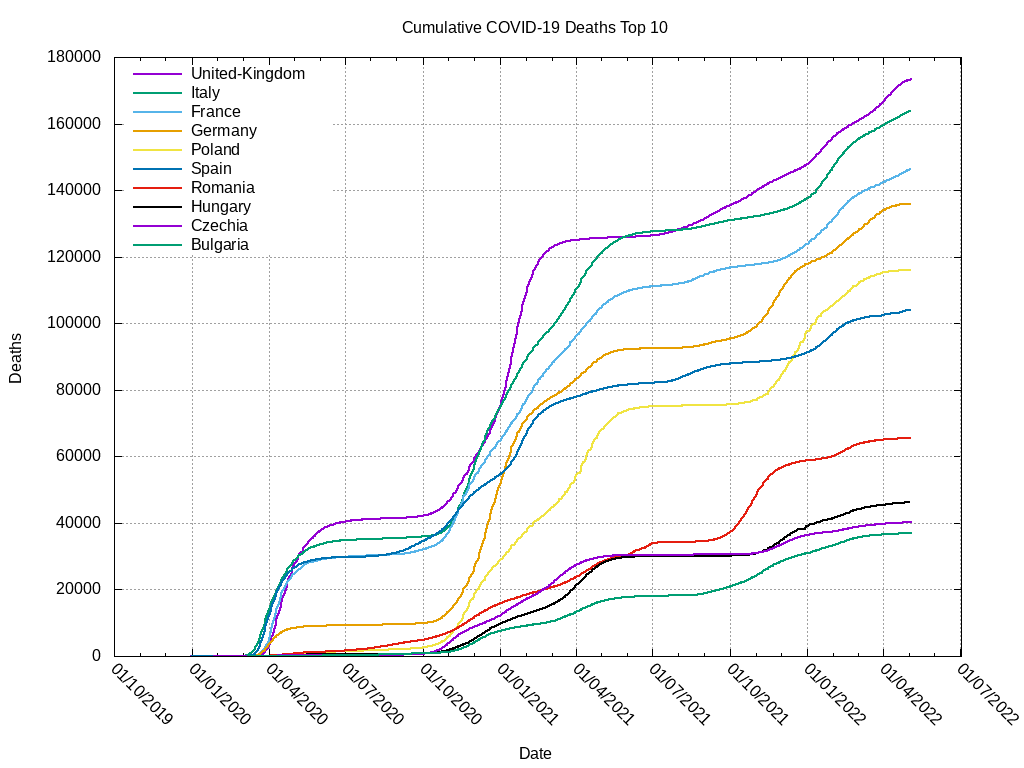
\includegraphics[width=1\linewidth]{graph.png}
\captionof{figure}{plot.sh resulting graph}

\end{document}
